%-----------------------------------------------------------------------------------
%	PACKAGES AND OTHER DOCUMENT CONFIGURATIONS
%----------------------------------------------------------------------------------



\documentclass[11pt]{article}

\usepackage[top=2cm, bottom=3cm, left=2cm, right=2cm]{geometry}

\setlength{\parindent}{0in}

\newcommand{\Var}{\mathrm{Var}}

\newcommand{\Cov}{\mathrm{Cov}}

\newcommand{\plim}{\rightarrow_{p}}

\usepackage{amsmath, amsfonts}
\usepackage{graphicx}
\usepackage{pdfpages}
\usepackage{bm}
\usepackage{listings}
\usepackage{multirow,array}
\usepackage{enumerate}
\usepackage{bbm}


\usepackage[latin1]{inputenc}

\usepackage{amssymb}

\usepackage{mathrsfs}
\usepackage{float}
\usepackage{booktabs}
\usepackage{color}
\usepackage{rotating}
\usepackage{amsthm}
\usepackage{multirow,array}
\usepackage{caption}
\usepackage{url}


\DeclareMathOperator*{\argmax}{arg\,max}
\DeclareMathOperator*{\argmin}{arg\,min}



% Expectation symbol
\newcommand{\E}{\mathrm{E}}
\newcommand{\V}{\mathrm{V}}
\newcommand{\N}{\mathcal{N}}
\newcommand{\R}{\mathbb{R}} 

%----------------------------------------------------------------------------------
%	TITLE AND AUTHOR(S)
%----------------------------------------------------------------------------------

\title{Econ 675 Assignment 1} % The article title


\author{Nathan Mather\thanks{Shouts out to Ani, Paul, Tyler, Erin, Caitlin and others for all the help with this } } % The article author(s) 

\date{\today} % An optional date to appear under the author(s)


%----------------------------------------------------------------------------------
\begin{document}
	
%------------------------------------------------------------------------------
%	TABLE OF CONTENTS & LISTS OF FIGURES AND TABLES
%------------------------------------------------------------------------------
\maketitle % Print the title/author/date block

\setcounter{tocdepth}{2} % Set the depth of the table of contents to show sections and subsections only

\tableofcontents % Print the table of contents


%-------------------------------------------------------------
% Question 1 
%-------------------------------------------------------------
\section{Question 1: Non-linear Least Squares}
\subsection{Q1 Part 1}

The general non-linear least squares estimator is 
$$ \bm{\hat{\beta}}_n = \arg \min_{\bm{\beta} \in \R^d} \frac{1}{n} \sum_{i=1}^{n}(y_i - \mu(\bm{x_i' \beta}))^2
$$

Now for $  \bm{\beta}_0 = \arg \min_{\bm{\beta} \in \R^d} \E[ (y_i - \mu(\bm{x_i' \beta}))^2]$ to be identifiable we need:

$$ \bm{\beta}_0 =  \bm{\beta}_0^* $$



$$ \iff  \bm{\beta}^*_0 = \arg \min_{\bm{\beta} \in \R^d} \E[ (y_i - \mu(\bm{x_i' \beta}))^2]$$ 

To find this start by noting that 

$$ \E[(y_i - \mu(\bm{x}'_i\bm{\beta}))^2] = \E[(y_i-\mu(\bm{x}'_i\bm{\beta}_0) +\mu(\bm{x}'_i\bm{\beta}_0) -\mu(\bm{x}'_i\bm{\beta})  )^2]
$$

$$ = \E[(y_i-\mu(\bm{x}'_i\bm{\beta}_0))^2] + \E[(\mu(\bm{x}'_i\bm{\beta}_0) -\mu(\bm{x}'_i\bm{\beta}) )^2] + 2\E[(y_i-\mu(\bm{x}'_i\bm{\beta}_0))(\mu(\bm{x}'_i\bm{\beta}_0) -\mu(\bm{x}'_i\bm{\beta})) ]
$$

$$
=\E[(y_i-\mu(\bm{x}'_i\bm{\beta}_0))^2] + \E[(\mu(\bm{x}'_i\bm{\beta}_0) -\mu(\bm{x}'_i\bm{\beta}) )^2]
$$

The last equality comes from the last term being zero by iterated expectations. I show this below. 

$$
\E[(y_i-\mu(\bm{x}'_i\bm{\beta}_0))(\mu(\bm{x}'_i\bm{\beta}_0) -\mu(\bm{x}'_i\bm{\beta}))] = \E[\E[(y_i-\mu(\bm{x}'_i\bm{\beta}_0))(\mu(\bm{x}'_i\bm{\beta}_0) -\mu(\bm{x}'_i\bm{\beta})) ]| \bm{x}_i]
$$

$$
= \E[(\E[y_i| \bm{x}_i]-\mu(\bm{x}'_i\bm{\beta}_0))(\mu(\bm{x}'_i\bm{\beta}_0) -\mu(\bm{x}'_i\bm{\beta}))] = 0
$$

Using this fact we have that 

$$
\E[(y_i - \mu(\bm{x}'_i\bm{\beta}))^2] =\E[(y_i-\mu(\bm{x}'_i\bm{\beta}_0))^2] + \E[(\mu(\bm{x}'_i\bm{\beta}_0) -\mu(\bm{x}'_i\bm{\beta}) )^2] \geq\E[(y_i-\mu(\bm{x}'_i\bm{\beta}_0))^2]
$$

$$ \forall \bm{\beta} \neq \bm{\beta}_0
$$

This is strictly greater than unless $\exists \bm{\beta} \neq \bm{\beta}_0 $ such that $\E[(\mu(\bm{x}'_i\bm{\beta}_0) -\mu(\bm{x}'_i\bm{\beta}) )^2] = 0 $ Thus this give us an identification condition that $\E[(\mu(\bm{x}'_i\bm{\beta}_0) -\mu(\bm{x}'_i\bm{\beta}) )^2] \neq 0$ $\forall \bm{\beta} \neq \bm{\beta}_0 $. This means that $\bm{\beta}_0$ is the unique minimizer of $\E[ (y_i - \mu(\bm{x_i' \beta}))^2]$

Next note that if $\mu(\cdot)$ is a linear function, $\bm{\beta}_0$ is the coefficient of the best linear predictor and has the usual closed form $\bm{\beta}_0 = \E[\bm{x}_i \bm{x}'_i]^{-1} \E[\bm{x}_i y_i]
$

\subsection{Q1 Part 2}

In order to set this up as a Z estimator lets take a first order condition. This gives use the following condition. 

$$ \E[(\mu(\bm{x}'_i\bm{\beta}_0) - \mu(\bm{x}'_i \bm{\beta})) \dot{\mu}(\bm{x}'_i\bm{\beta})\bm{x}_i] = 0 
$$

Now take the sample analog and let $m(\bm{z}_i, \bm{\beta}) = (y_i - \mu(\bm{x}'_i \bm{\beta})) \dot{\mu}(\bm{x}'_i\bm{\beta})\bm{x}_i $ where $\bm{z}_i = (y_i, \bm{x}'_i)'$. We can write $\hat{\bm{\beta}}_n$ as the Z-estimator that solves:

$$ 0 = \frac{1}{n} \sum_{i=1}^{n} m(\bm{z}_i, \hat{\bm{\beta}}_n)
$$

Now assuming $ \hat{\bm{\beta}}_n \to \bm{\beta}_0 $ and regularity conditions we get the standard M estimation result.

$$ \sqrt{n}(\hat{\bm{\beta}}_n - \bm{\beta}_0) \to_d \N(0, \bm{H_0^{-1} \Sigma_0 H_0^{-1}})
$$ 
Were 
$$
\bm{H}_0 = \E \left[ \frac{\partial}{\partial \bm{\beta}} m(\bm{z}_i, \bm{\beta}_0) \right] = \E[ \dot{\mu}(\bm{x}'_i \bm{\beta}_0)^2\bm{x_ix'_i} ]
$$

and 
$$
\bm{\Sigma_0} = \V[m(\bm{z}_i, \bm{\beta}_0)] = \E[\sigma^2(\bm{x_i}) \dot{\mu}(\bm{x'_i \beta_o})^2 \bm{x_ix'_i}]
$$


\subsection{Q1 Part 3}

$$\hat{\V}_n^{HC} = \left( \frac{1}{n} \sum_{i=1}^{n} \hat{\bm{m}} \hat{\bm{m}}'  \right)^{-1}  \left( \frac{1}{n} \sum_{i=1}^{n} \hat{\bm{m}} \hat{\bm{m}}' \hat{e}_i^2  \right) \left( \frac{1}{n} \sum_{i=1}^{n} \hat{\bm{m}} \hat{\bm{m}}'  \right)^{-1} 
$$

where $\hat{\bm{m}} = \bm{m_{\beta}(z_i, \hat{\beta})} $  and $ hat{e} = y_i -\bm{m(z_i, \hat{\beta})} $

 Now by the delta method and letting $g(\bm{\beta}) = \lVert \bm{\beta} \rVert = \sum_{k=1}^{d} \bm{\beta}_k^2
$ we get 

$$ \sqrt{n}(g(\hat{\bm{\beta_n}}) - g(\bm{\beta}_0)) \to_d \N (0, \dot{g}(\bm{\beta}_0) \bm{V}_0 \dot{g}(\bm{\beta}_0)')
$$

where $\dot{g}(\bm{\beta}_0) = \frac{d}{d\bm{\beta}'}g(\bm{\beta}) = 2 \bm{\beta}' $ Hence the confidence interval is given by 


$$ CI_{0.95} = \left[ \lVert \hat{\bm{\beta}}_n \rVert ^2 - 1.96 \sqrt{\frac{4\hat{\bm{\beta_n}}'\hat{\bm{V}} \hat{\bm{\beta_n}} }{n}},  \lVert \hat{\bm{\beta}}_n \rVert ^2 + 1.96 \sqrt{\frac{4\hat{\bm{\beta_n}}'\hat{\bm{V}} \hat{\bm{\beta_n}} }{n}} \right] 
$$


\subsection{Q1 Part 4}

In this case we get $\bm{\Sigma_0} = \sigma^2 \bm{H}_0$ and the asymptotic variance reduces to 

$$ \bm{V}_0 = \sigma^2 \bm{H}_0 ^{-1} = \sigma^2 \E[ \dot{\mu}(\bm{x}'_i \bm{\beta}_0)^2\bm{x_ix'_i} ]^{-1} $$

We can estimate variane using $\hat{\bm{V}} = \hat{\sigma}^2 \hat{\bm{H}}^{-1}$ where 

$$ \hat{\sigma}^2 = \frac{1}{n} \sum_{i=1}^{n}(y_i - \mu(\bm{x}'_i \hat{\bm{\beta}}_n))^2
$$
and 
$$ \hat{\bm{H}} = \frac{a}{n} \sum_{i=1}^{n}\dot{\mu}(\bm{x}'_i \bm{\beta}_0)^2\bm{x_ix'_i}
$$

Which is consistent by the continuous mapping theorem. Now by the delta method and letting $g(\bm{\beta}) = \lVert \bm{\beta} \rVert = \sum_{k=1}^{d} \bm{\beta}_k^2
$ we get 

$$ \sqrt{n}(g(\hat{\bm{\beta_n}}) - g(\bm{\beta}_0)) \to_d \N (0, \dot{g}(\bm{\beta}_0) \bm{V}_0 \dot{g}(\bm{\beta}_0)')
$$

where $\dot{g}(\bm{\beta}_0) = \frac{d}{d\bm{\beta}'}g(\bm{\beta}) = 2 \bm{\beta}' $ Hence the confidence interval is given by 


$$ CI_{0.95} = \left[ \lVert \hat{\bm{\beta}}_n \rVert ^2 - 1.96 \sqrt{\frac{4\hat{\bm{\beta_n}}'\hat{\bm{V}} \hat{\bm{\beta_n}} }{n}},  \lVert \hat{\bm{\beta}}_n \rVert ^2 + 1.96 \sqrt{\frac{4\hat{\bm{\beta_n}}'\hat{\bm{V}} \hat{\bm{\beta_n}} }{n}} \right] 
$$

\subsection{Q1 Part 5}
The conditional likelihod funciton is 

$$f_{y|x}(y_i|\bm{x}_i) = \frac{1}{(2\pi)^{n/2} \sigma^2} exp \left( -\frac{1}{2 \sigma^2} \sum_{i=1}^{n}(y_i - \mu(\bm{x}_i'\bm{\beta}))^2 \right)
$$

with log likelihood 

$$ \ell_n(\bm{\beta}, \sigma^2) = -\frac{1}{2\sigma^2} \sum_{i=1}^{n}(y_i - \mu(\bm{x}_i' \bm{\beta}))^2 - \frac{n}{2}log(\sigma^2)
$$

This gives us the following first order conditions 

$$ \frac{\partial}{\partial \bm{\beta}} \ell_n(\bm{\beta}, \sigma^2) = \frac{1}{\hat{\sigma}_{ML}^2} \sum_{i=1}^{n}(y_i - \mu(\bm{x}_i' \bm{\beta}_{ML}))\dot{\mu}(\bm{x}_i' \bm{\beta}_{ML})\bm{x}_i = 0
$$

$$\frac{\partial}{\partial \sigma^2} \ell_n(\bm{\beta}, \sigma^2) =
\frac{1}{2\hat{\sigma}_{ML}^4} \sum_{i=1}^{n}(y_i - \mu(\bm{x}_i' \bm{\beta}_{ML}))^2 - \frac{n}{2 \hat{\sigma}_{ML}^2} =0
$$

These conditions are equivalent to those found above. 

\subsection{Q1 Part 6}
If the link funciton is unknown, $\bm{\beta}_0$ is not identified. To see this, consider two pairs of parameters $(\mu(\cdot), \bm{\beta}_0)$ and $(\tilde{\mu}(\cdot), \tilde{\bm{\beta}}_0)$ where $\tilde{\mu}(z) = \mu(z/k)$ and $\tilde{\bm{\beta}}_0 = k\bm{\beta}_0$ for some $ k \ne 0$. Then the parameters are clearly different, but $(\mu(\cdot), \bm{\beta}_0) = (\tilde{\mu}(\cdot), \tilde{\bm{\beta}}_0)$. A common normalization is $\lVert \bm{\beta}_0 \rVert = 1$, but more conditions are needed to regain identification.

\subsection{Q1 Part 7}
The link function is 
$$\mu(\bm{x}'_i \bm{\beta}_0) = \E[y_i|\bm{x}_i] = \E[\mathbbm{1}(\bm{x}'_i \bm{\beta}_0 \geq \epsilon_i)|\bm{x}_i] =Pr[\bm{x}'_i \bm{\beta}_0 \geq \epsilon_i|\bm{x}_i] = F(\bm{x}'_i \bm{\beta}_0) = \frac{1}{1+exp(-\bm{x}'_i \bm{\beta}_0)}
$$
\subsection{Q1 Part 8}



\subsection{Q1 Part 9 }
(a)\\

\centerline{R table }

\begin{center}
	% latex table generated in R 3.3.2 by xtable 1.8-2 package
% Sun Oct 28 23:39:33 2018
\begin{tabular}{lrrrrrr}
  \hline
term & estimate & std.error & statistic & p.value & CI\_L & CI\_H \\ 
  \hline
(Intercept) & 1.755 & 0.335 & 5.245 & 0.000 & 1.099 & 2.411 \\ 
  S\_age & 1.333 & 0.123 & 10.826 & 0.000 & 1.092 & 1.575 \\ 
  S\_HHpeople & -0.067 & 0.023 & -2.871 & 0.004 & -0.112 & -0.021 \\ 
  log\_inc & -0.119 & 0.044 & -2.707 & 0.007 & -0.205 & -0.033 \\ 
   \hline
\end{tabular}

\end{center}



(b)

\centerline{R table }

\begin{center}
	% latex table generated in R 3.3.2 by xtable 1.8-2 package
% Sat Oct 27 23:36:46 2018
\begin{tabular}{lrrrrrr}
  \hline
term & estimate & std.error & t\_q.975 & t\_q.025 & CI\_L & CI\_H \\ 
  \hline
(Intercept) & 1.755 & 0.335 & 2.167 & -1.774 & 1.161 & 2.480 \\ 
  S\_HHpeople & -0.067 & 0.023 & 2.040 & -1.958 & -0.112 & -0.019 \\ 
  S\_age & 1.333 & 0.123 & 2.210 & -1.558 & 1.142 & 1.606 \\ 
  log\_inc & -0.119 & 0.044 & 1.817 & -2.155 & -0.213 & -0.039 \\ 
   \hline
\end{tabular}

\end{center}


(c)
\centerline{R Graph }
\begin{center}
	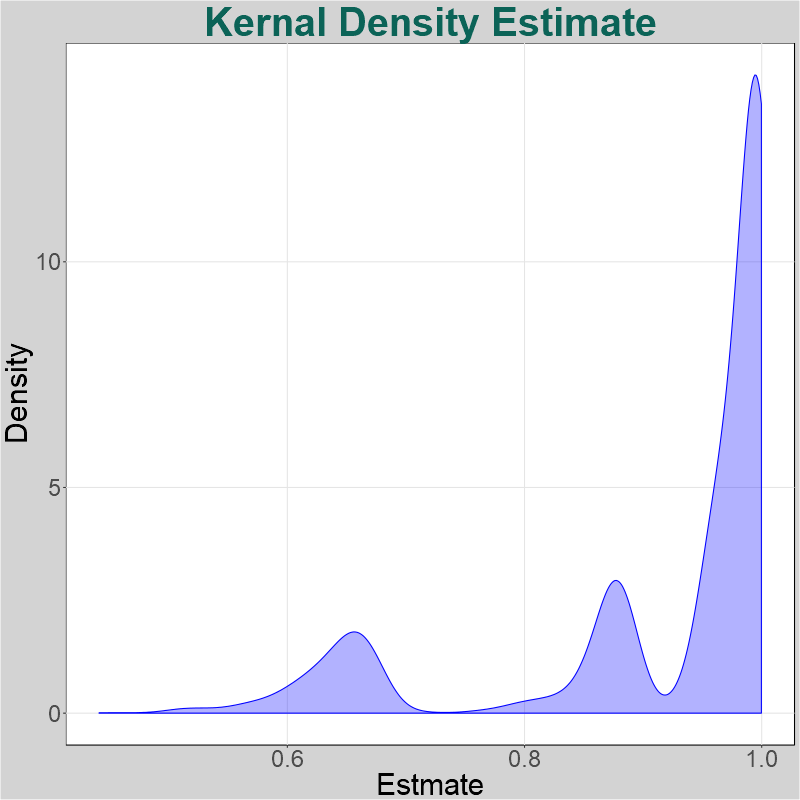
\includegraphics[width=.8\linewidth]{plot_q1_9_c.png}
	
\end{center}


% -----------------------------------------------------
% QUESTION 2
%------------------------------------------------------

\section{Question 2: Semiparametric GMM with Missing Data}
\subsection{Q2 part 1}

Start with the moment condition we are given
$$
0 = \mathbb{E}[m(y_i^*, t_i, x_i; \beta_0)|t_i,x_i] $$

Now by law of iterated expectations we can multiply by a function g and still get zero
$$ 0 = \mathbb{E}[g(t_i, x_i)\mathbb{E}[m(y_i^*, t_i, x_i; \beta_0)|t_i, x_i]] \text{ for any } g(t_i, x_i) $$

Next we can put g inside the first expectation
$$ 0 = \mathbb{E}[\mathbb{E}[g(t_i, x_i)m(y_i^*, t_i, x_i; \beta_0)|t_i, x_i]] $$

now removing the inside expectation 
$$ 0 = \mathbb{E}[g(t_i, x_i)m(y_i^*, t_i, x_i; \beta_0)]$$

We want to find $g_0$, the optimal $g$ that minimizes AsyVar($\hat{\beta}$). Let $z_i=(t_i,x_i)$, $w_i = (y_i^*,t_i,x_i)$, and $\theta=\beta$.
\\ \\ 
The first thing we need to do is determine the asymptotic variance V associated with 


$$\hat{\theta} = \argmin (\frac{1}{n}\sum_i g(z_i)m(w_i,\theta))'W(\frac{1}{n}\sum_i g(z_i)m(w_i,\theta))$$

Taking first order conditions and setting equal to zero we get 

$$\text{FOC: } 0 = [\frac{1}{n}\sum_i \frac{\partial}{\partial\theta}g(z_i)m(w_i,\theta)]'W[\frac{1}{n}\sum_i \frac{\partial}{\partial\theta}g(z_i)m(w_i,\theta)]$$

or 
$$ 0 = [\frac{1}{n}\sum_i \frac{\partial}{\partial\theta}g(z_i)m(w_i,\hat{\theta})]'W[\frac{1}{n}\sum_i \frac{\partial}{\partial \theta}g(z_i)m(w_i,\hat{\theta})]$$

Since it is euqual to zero we can add another of the same term and multiply by $(\hat{\theta}-\theta_0)$ giving 

$$0 = [\frac{1}{n}\sum_i \frac{\partial}{\partial\theta}g(z_i)m(w_i,\theta_0)]'W[\frac{1}{n}\sum_i \frac{\partial}{\partial \theta}g(z_i)m(w_i,\theta_0)] + [\frac{1}{n}\sum_i \frac{\partial}{\partial\theta}g(z_i)m(w_i,\hat{\theta})]'W[\frac{1}{n}\sum_i \frac{\partial}{\partial \theta}g(z_i)m(w_i,\hat{\theta})](\hat{\theta}-\theta_0)$$

Which can be rearanged to give 

$$\sqrt n(\hat{\theta}-\theta_0) = (\Omega_0'W_0\Omega_0)^{-1}\Omega_0W_0\frac{1}{\sqrt n}\sum_i g(z_i)m(w_i,\theta) + o_p(1)$$

And then  By the CLT, $\sqrt n(\hat{\theta}-\theta_0) \rightarrow_d N(0,V_0)$ \\ \\
where $ V_0 = (\Omega_0'W_0\Omega_0)^{-1}\Omega_0'W_0\Sigma_0W_0\Omega_0(\Omega_0'W_0\Omega_0)^{-1}$\\ \\ 

and where $ \Sigma_0 = \mathbb{V}[g(z_i)m(w_i,\theta)]$


 setting values Optimally to minimize V gives us the following conditions. 
 
 $$ W_0^* = \Sigma_0^{-1} \text{ and } V_0^* = \Omega_0'\Sigma_0\Omega_0$$

$$g^*(z_i) = \frac{\partial m_i}{\partial \theta} \mathbb{V}[m(w_i,\theta_0)|z_i]^{-1} $$


Now applying this specifically to a probit model gives 
$$ \mathbb{V}[m(y_i^*,t_i,x_i,\beta_0)|t_i,x_i]=F(t_i \cdot \theta_0+x_i\gamma_0)(1-F(t_i \cdot \theta_0 + x_i'\gamma_0))$$

$$\mathbb{E}[\frac{\partial}{\partial \beta}m(y_i^*,t_i,x_i,\beta_0)|t_i,x_i] = \mathbb{E}[f(t_i \cdot \theta_0+x_i\gamma_0)(t_i,x_i)|t_i,x_i]
= f(t_i \cdot \theta_0+x_i\gamma_0)[t_i,x_i']'$$

$$\text{Therefore, } g_0(t_i,x_i) = \frac{f(t_i \cdot \theta_0+x_i\gamma_0)}{F(t_i \cdot \theta_0+x_i\gamma_0)(1-F(t_i \cdot \theta_0 + x_i'\gamma_0))}[t_i,x_i']'$$


If $F$ is the logistic cdf we instead get 
\begin{align*}
F(x) = \frac{1}{1+e^{-x}}\\
f(x) = \frac{\partial}{\partial x}F(x) = \frac{-e^{-x}}{(1+e^{-x})^2} =-e^{-x}F(x)^2\\
\frac{f(x)}{F(x)(1-F(x))} = \frac{-e^{-x}F(x)^2}{F(x)(1-F(x))} = \frac{-e^{-x}F(x)}{1-F(x)} = 1 \\
g_0(t_i,x_i) = [t_i,x_i']'
\end{align*}

\subsection{Q2 part 2}
\begin{enumerate}[(a)]
	\item The optimal unconditional moment condition is:
	\begin{align*}
	0 = \mathbb{E}[g(t_i, x_i)m(y_i^*, t_i, x_i; \beta_0)]
	\end{align*}
	In part 2.1 we showed that, setting $g=g_0$ this is equivalent to:
	\begin{align*}
	0 = \mathbb{E}[m(y_i^*, t_i, x_i; \beta_0)|t_i,x_i]
	\end{align*}
	Since $s_i  \perp (y_i^*,t_i,x_i)$:
	\begin{align*}
	0 = \mathbb{E}[m(y_i^*, t_i, x_i; \beta_0)|t_i,x_i]\\
	0 = \mathbb{E}[g_0(t_i, x_i)m(y_i^*, t_i, x_i; \beta_0)]\\
	0 = \mathbb{E}[g_0(t_i, x_i)m(y_i^*, t_i, x_i; \beta_0) | s_i=1]
	\end{align*}
	Thus, $\hat{\beta}_{MCAR}$ solving $0 \approx \hat{\mathbb{E}}[g_0(t_i,x_i)m(y_i, t_i, x_i; \hat{\beta}_{MCAR})|s_i=1]$ is consistent for $\beta_0$\\
	$\hat{\beta}_{MCAR,feasible}$ solves $0 \approx \hat{\mathbb{E}}[\hat{g}(t_i,x_i)m(y_i, t_i, x_i; \hat{\beta}_{MCAR})|s_i=1]$
	
	\item The tables for this section are below \\
	
	\centerline{R table }
	\begin{center}
		% latex table generated in R 3.3.2 by xtable 1.8-2 package
% Sat Oct 27 23:36:46 2018
\begin{tabular}{lrrrrrr}
  \hline
term & Estimate & sd & p\_value & t & CI\_L & CI\_H \\ 
  \hline
dpisofirme & -0.317 & 0.073 & 0.008 & -4.363 & -0.453 & -0.187 \\ 
  S\_age & -0.244 & 0.020 & 0.000 & -11.975 & -0.284 & -0.205 \\ 
  S\_HHpeople & 0.024 & 0.013 & 0.104 & 1.775 & -0.002 & 0.049 \\ 
  log\_inc & 0.033 & 0.014 & 0.020 & 2.397 & 0.006 & 0.058 \\ 
   \hline
\end{tabular}

	\end{center}
	
\end{enumerate}

%--------------------------------------------------------
% Question 3 
%--------------------------------------------------------

\section{Question 3: When Bootstrap Fails}
\subsection{Q3 part 1}
\centerline{R Graph }
\begin{center}
	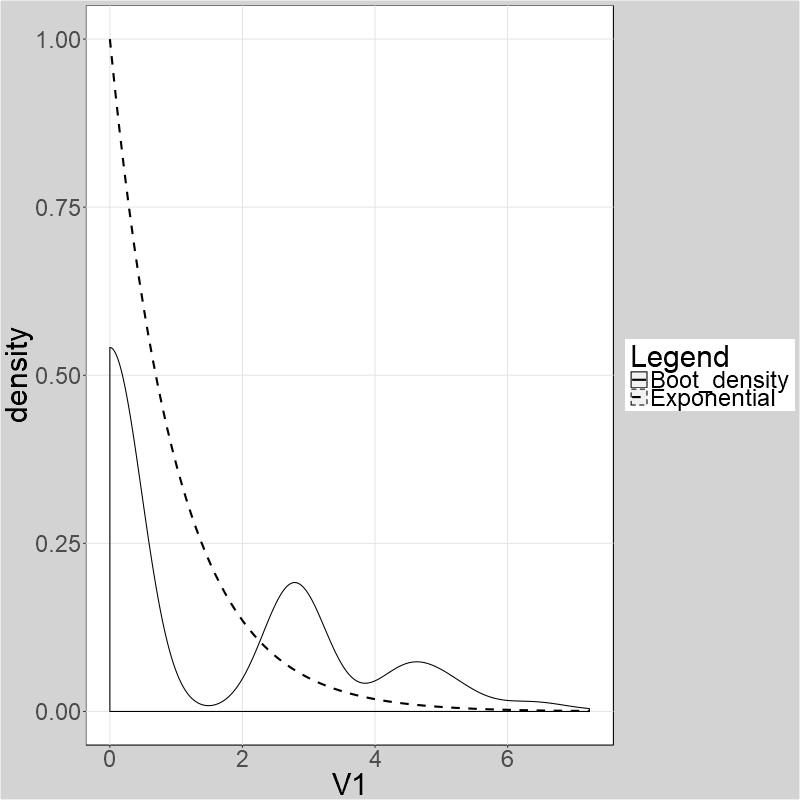
\includegraphics[width=.8\linewidth]{plot_q3_1.png}	
\end{center}


\subsection{Q3 part 2}
\centerline{R Graph }
\begin{center}
	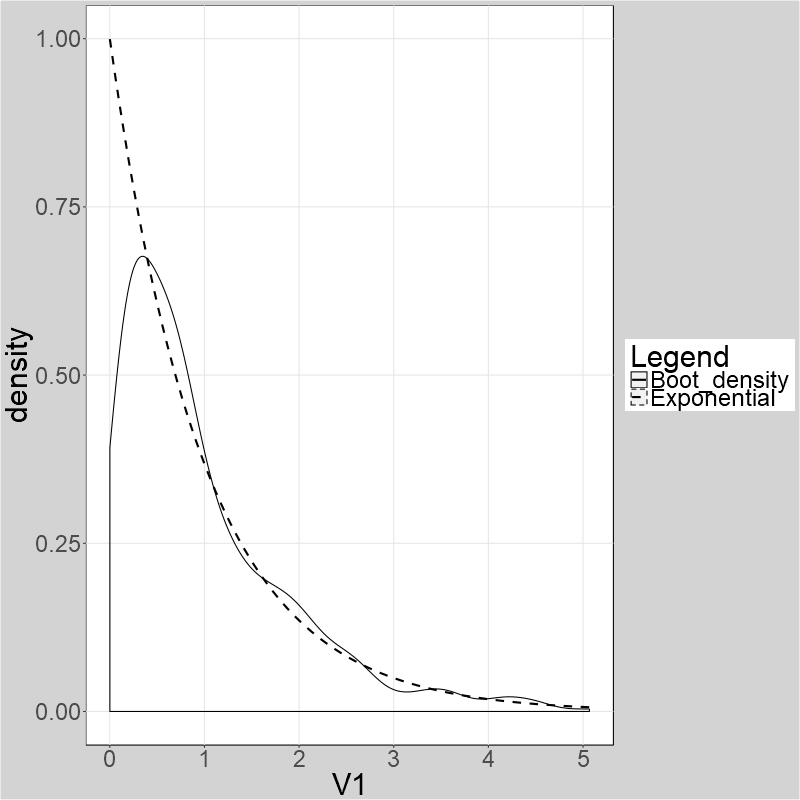
\includegraphics[width=.8\linewidth]{plot_q3_2.png}	
\end{center}

\subsection{Q3 part 3}
In the nonparametric case, the bootstrap statistic has a mass point at zero. However, the parametric bootstrap corrects for this since $Pr[max\{x_i\} = max\{x_i^*\}] = 0$, since $x_i^* \sim_{iid} Uniform[0,maz\{x_i\}]$
%------------------------------------------------
% end doc
%------------------------------------------------
\end{document}

